% !TeX root = ../main.tex

\chapter{研究方法}

本研究提出一個基於知識本體的語意位置描述三層式架構(ontology based semantic location description framework, O-SLD framework),旨在整合空間資料與自然語言中的位置描述語意,建構具有語意表達能力的位置描述之知識模型。透過本框架,期望為位置描述中的語意提供形式化模型,並強化空間資料、空間認知與自然語言之間的語意連結與互通性。在3.1節中,說明位置描述語意(O-SLD)三層式架構之設計,以達成空間資料、位置語意與位置詞彙的連結;在3.2節說明位置描述知識本體建構原則與內容架構;在3.3節描述規則設計準則及機制,以實現語意式位置描述的動態產生能力;在3.4節說明本研究評估方法,將採用SPICE(Semantic Propositional Image Caption Evaluation)作為評估指標。

\section{位置描述語意(O-SLD)三層式架構設計}

為回應空間認知理論對人類位置理解的需求,並解決位置描述語意表徵上的挑戰,本研究設計了O-SLD三層式架構。該框架透過語意推理機制,能進一步從空間資料產生位置語意及語意式位置描述,能達成逆向地理編碼任務。框架的結構如\ref{fig:three-layered}所示,O-SLD三層式架構主要由三個層級組成:資料層、語意層和自然語言層。三層之間呈現自上而下的語意映射關係,分別對應空間資料、知識本體與語言表達,透過語意規則加以串連各層級,形成完整的語意推論機制。

\begin{figure}[!htbp]
\centering
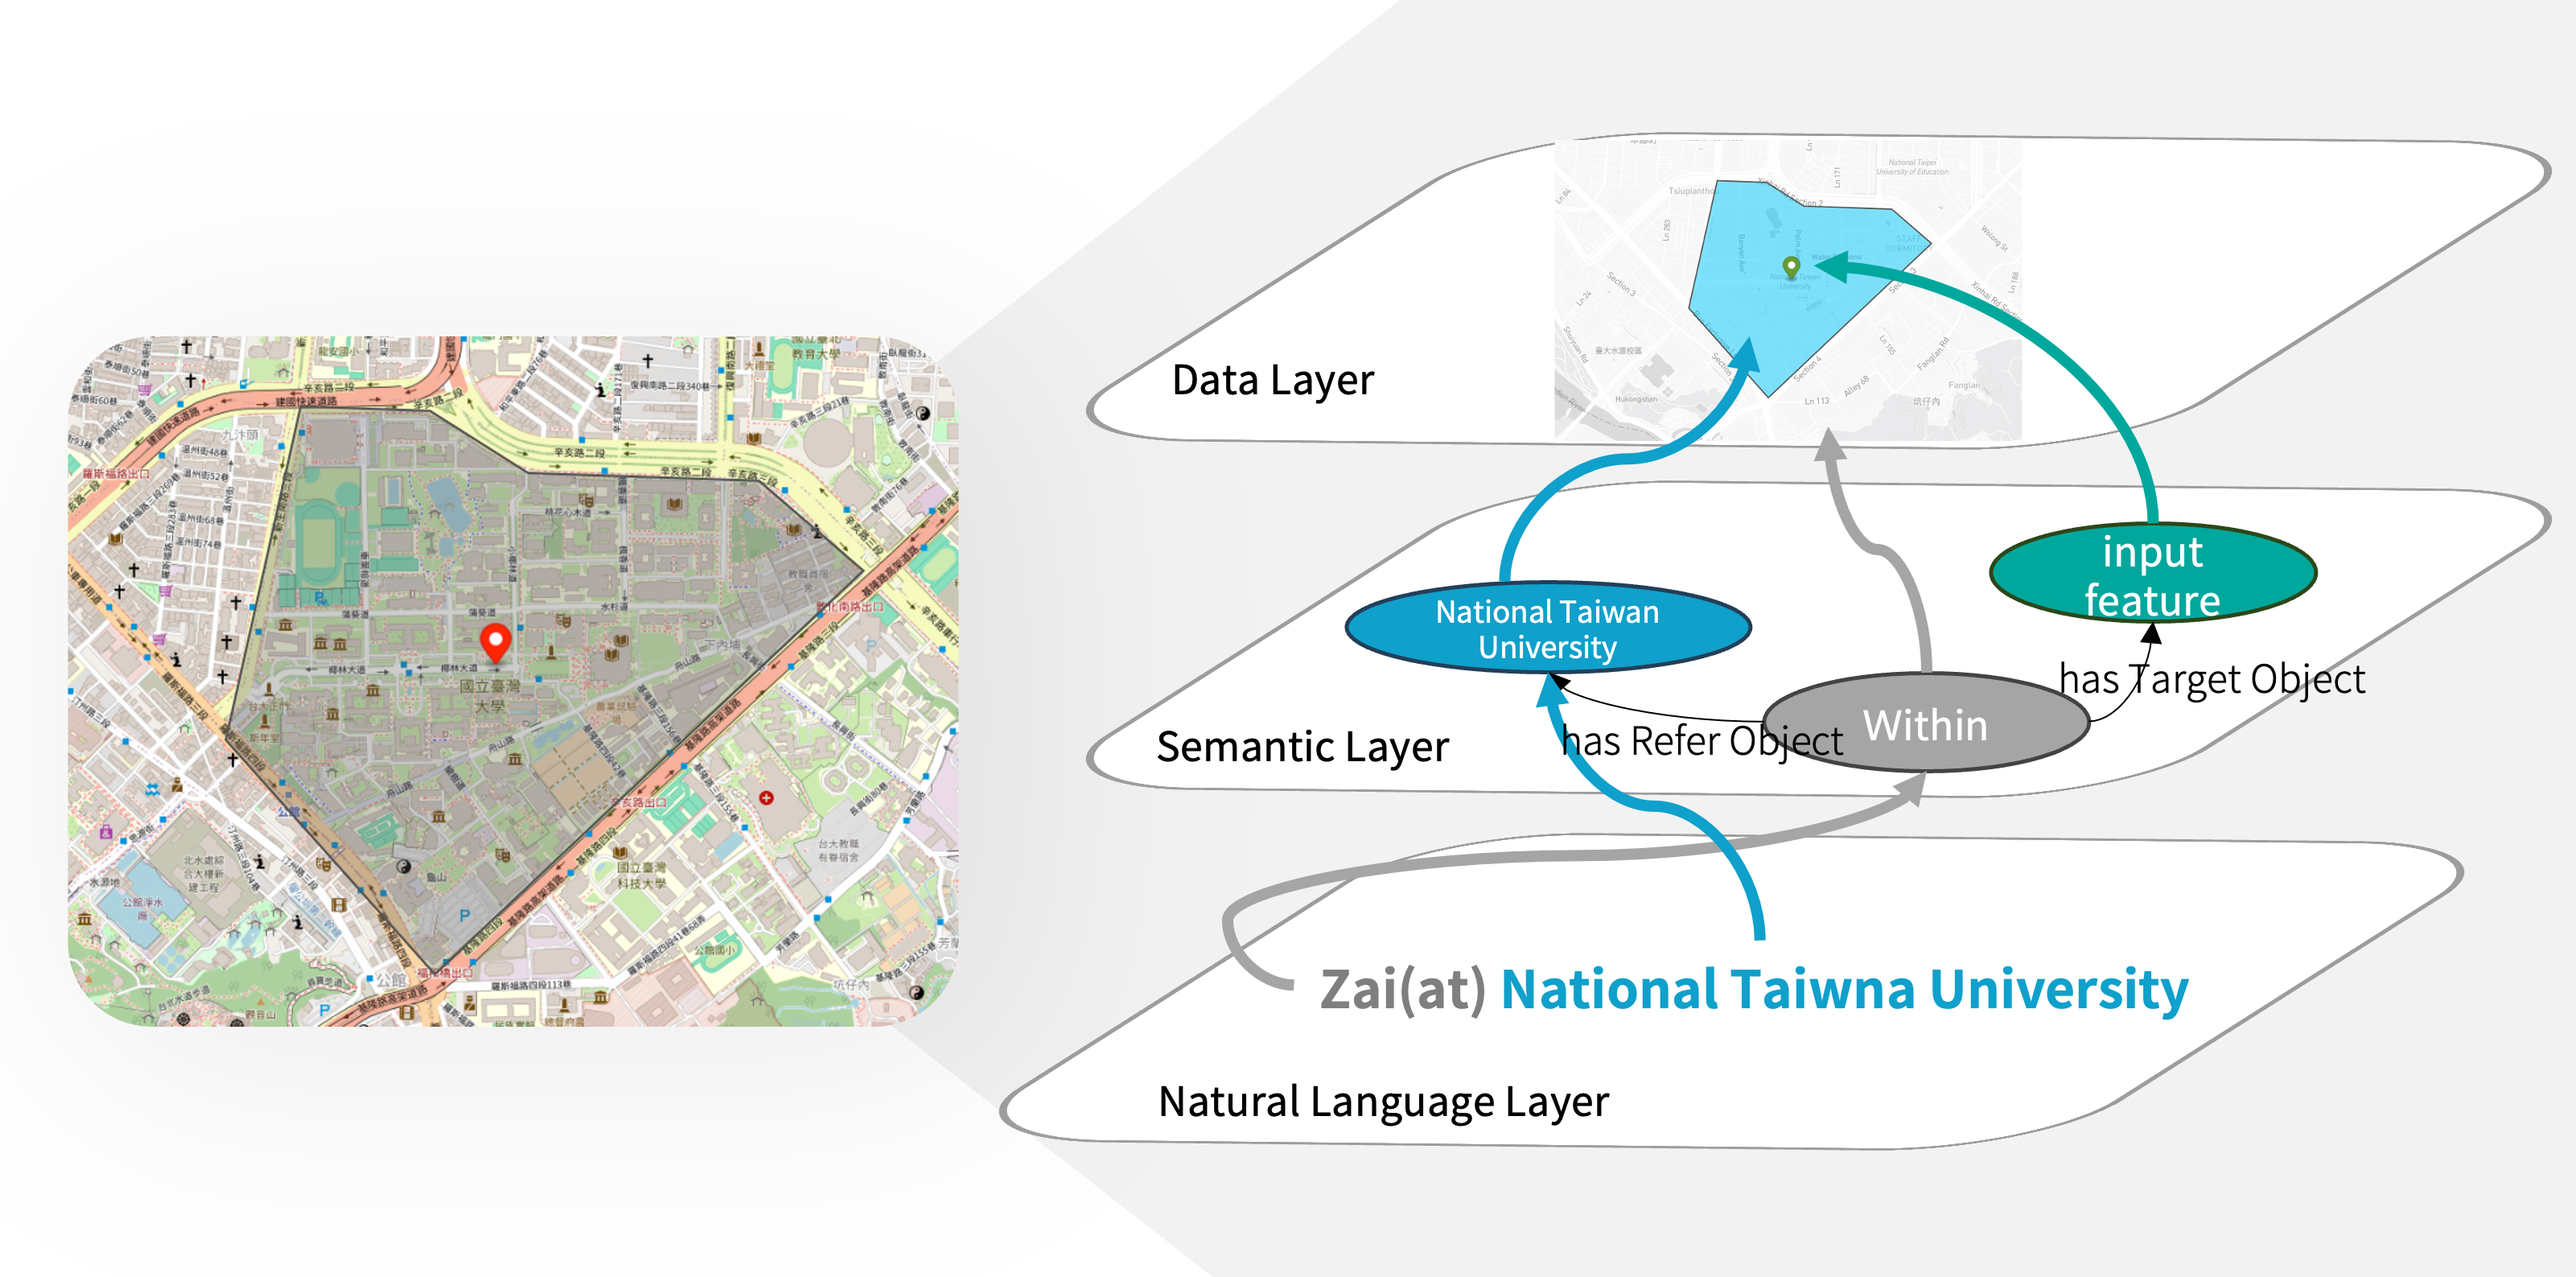
\includegraphics[width = \textwidth]{figures/three-layered.png}
\caption{位置描述語意三層式架構}
\label{fig:three-layered}
\end{figure}

「資料層」主要負責空間資料的紀錄與關係操作,包括點、線和面等的GIS Feature,以及其屬性與彼此間的空間關係。本研究將資料層獨立設計,旨在提供全面且詳盡的空間資料表示,支持進階的空間關係建模與語意推理。該層作為框架的基礎,為後續語意層與自然語言層提供圖資、詮釋資料及空間操作。

而「語意層」是框架的核心,負責知識本體的語意表徵與知識整合,透過知識本體存有形式化的特性,可整合來自GIS、空間認知和語言學等多領域的位置相關知識,支持位置語意的建構和語意位置描述的產生。本層的知識本體設計具有高可擴展性,能夠隨研究目標需求進一步擴充,從而豐富語意資訊。作為框架的中介層,語意層透過規則建構與推理機制,實踐各層級之間的互動,包含語意空間關係的推理及產生位置描述文字等。

最後,「自然語言層」負責將語意層中的知識與推理結果轉化為人類可讀之自然語言文本,並透過語言樣板與結構設定呈現自然語言式的位置描述給使用者。

本研究所提出之O-SLD三層式架構可應用於逆向地理編碼機制,能根據使用者輸入坐標位置,自動檢索並產生產生語意式位置描述。其核心功能在於:透過語意推理機制,將空間資料轉換為具有語意的知識表徵,進而轉譯成人類可理解之文字表達,從而促進使用者對位置之所在的理解與日常應用。以圖 2所示,當輸入點查詢位置描述時,機制參考各類參考物,並與之產生空間關係,詳細流程如下:首先,資料層到語意層的推論過程,判斷輸入圖徵與資料層中給定的各類參考物圖徵(如建物、行政區或地標等)之空間關係。若該點落在「台灣大學」這一圖徵內,則推論該點與「台灣大學」具有「位於(Within)」之空間關係,並將該資訊納入知識本體。接著,在語意層到自然語言層的過程,根據產生一組包含參考圖徵之語意及空間關係的知識本體,根據語料庫的規則進一步執行語意推論機制。最終,選擇情境下的語言樣板,產生對應到自然語言式之文字。例如,產生「在台灣大學」這一語意式位置描述。因此,結合O-SLD三層式架構可有效進行知識獲取與創造,進而轉換為文字式的位置描述。

\section{位置描述知識本體(location description ontology, LocD)}

本研究採用常見的知識本體建構過程METHONTOLOGY\citep{RN143},其建構過程包含需求規範、知識獲取、概念化、整合、實作與評估等七個階段,用以建立任務為導向的位置描述知識本體(LocD)。

本節首先說明所使用之上層知識本體,以提供在語意領域中整合基礎及互通能力,亦能有效降低語意重複與歧異產生。其次,說明位置描述知識本體中兩個子集結構:「圖徵及性質」和「位置描述與空間概念」。前者對應O-SLD三層式架構中的「資料層」,旨在定義空間資料如何介接知識本體,例如「台灣大學」作為Feature,存在幾何類型—「面」、名稱—「台灣大學」和類型—「大學」等資訊,這些資訊將分別記錄於「圖徵與性質」之子集中。同時,輸入圖徵與參考圖徵產生的空間操作(spatial operation)結果也將記錄於其下;後者則對應O-SLD三層式架構中的「自然語言層」,旨在定義位置描述語言中的空間介詞與方位詞,並賦予其對應之語意空間關係。這些語意元素分別記錄在「位置描述與空間概念」之子集中,進一步支持位置描述文字的語意。

\subsection{上層知識本體}

達成語意互通,本研究採用三個上層知識本體框架進行知識本體建構的整合既有知識(如圖3所示),分別為:Descriptive Ontology for Linguistic and Cognitive Engineering (DOLCE)、GeoSPARQL Ontology和廣義知網知識本體(Extended-HowNet Ontology, E-HowNet ontology)。位置描述的產生過程以空間認知的三個核心概念構成其基本結構,分別為Feature (\textit{dul:Feature})、空間概念(\textit{locd:SpatialConcept})及位置描述(\textit{locd:LocationDescription})。此外,形塑空間概念的組成元素則記錄於性質(\textit{dul:Quality})之下,使得知識本體可涵蓋空間認知過程形成位置描述的關鍵特徵,並有助於各個子類語意關係明確化。上層知識本體的引入,係基於該結構之考量,以下詳述個別內容:

\subsubsection{Descriptive Ontology for Linguistic and Cognitive Engineering (DOLCE)}

為建構具語意推理能力和整合不同領域的位置語意資訊的的位置描述知識本體,本研究採用經邏輯語言公理化(axiomatized)的上層知識本體 DOLCE作為語意架構基礎,其實體分類系統與性質描述機制可有效支持位置語意的建模與跨領域整合(參見圖4)。

DOLCE旨在基於認知和語言考量來建立一個人類日常所使用和理解的事物之常識模型作為一個基礎知識本體,核心目的是提供一般性的範疇和關係,以建構一個連貫的現實理解框架\citep{RN86}。同時,DOLCE已廣泛應用於社會技術系統、製造業、金融交易和文化遺產等領域,在地理資訊領域中,亦透過DOLCE建立跨領域術語與知識結構,支援不同領域間的語意中\citep{RN195, RN193}。

對應於人如何理解環境的過程,會存在物理的地理環境與抽象後的表徵(例如GIS上的Feature或文字式的位置描述),DOLCE的分類結構將實體第一階層區分為「Endurant(持續體)」和「Perdurant(發生體)」。Endurant指的是在任何存在的時間點,其所有部分都在,例如:一棟建築;反之Perdurant是部分臨時存在的,也就是在任何展開的時間點,只有一部分存在,例如:牆壁上的裂縫。

進一步地,第二層上Endurant又依其是否具備物理性質區分子類,分別為「Physical Endurant(物理持續體)」指的是具有具體的物理性質,和「Non-Physical Endurant(非物理持續體)」多指抽象的或社會性的實體,例如:「詞彙(word)」作為位置語意的語言表徵,屬於非物理持續體中的符號化實體;而「詞意(word sense)」作為語意,亦屬於非物理持續體中的抽象概念。在本研究發展之位置描述知識本體中,將Feature劃分為Physical Endurant,而其隱含的空間概念則是Non-Physical Endurant。以「台北101」為例,其可以是一個實際存在的物理空間特徵(為Physical Endurant),但在概念層次中則可能代表一個隱性的概念(為Non-Physical Endurant下的Concept),例如台灣的最高樓等。

此外,DOLCE 不僅關注於實體的分類,亦在Quality(性質)上提供完整的上層知識本體結構,使其能夠有效地描述可被感知與測量的東西與實體之間的依存關係,在本研究的任務中對應於Feature及其屬性資料,這一分類方法可應用於區分地理物件的測量屬性(如坐標值和樓高等)與其語意屬性(如類型、重要性和歷史文化價值等),進一步提升Feature的語意表達範疇。更詳細來說,性質被視為依附於特定實體的特徵,無法獨立存在。例如,「顏色」作為性質的一種,僅當它與某一物體(例如一棟建築)相關聯時,才具備語意價值。這種對於性質的描述,使得 DOLCE 能夠在語意推理中明確區分性質本身與其承載的實體。如同實體子類之區分,DOLCE將性質進一步區分為「Physical Quality(物理性質)」與「Abstract Quality(抽象性質)」,分別對應於具體可測量的屬性(如重量和長度等)與較抽象的特徵(如情緒和評價等)。

綜上所述,DOLCE 具備明確的分類體系與語意結構設計,能夠有效支援位置語意資訊的組織與推理。本研究將其作為核心上層知識本體,整合位置描述所需之Feature的語意、性質分類與空間概念,進一步推進跨領域語意理解與空間資料之結合,建立更具解釋性與可推理性的語意位置描述模型。

\subsubsection{GeoSPARQL Ontology}

為確保空間資料的可解釋性與可互操作性,本研究將 GeoSPARQL作為表達空間資料幾何特徵與空間操作的主要語意框架,並結合 DOLCE進一步提升位置語意推理的能力。

GeoSPARQL Ontology由開放地理空間協會(Open Geospatial Consortium, OGC)所制定的語意網標準,旨在表達空間資訊支援查詢與推理(參見圖 5)。其定義了「Feature(圖徵)」、「Geometry(幾何)」等類別,前者代表特定論域中的離散的空間現象,不論其是否有明確邊界,其皆具有可識別性,例如:行政區界、山脈及颱風等;而後者為在空間中一組連貫的直接位置,這些位置存在於空間參考系統內,用來表達Feature的幾何表現(例如形狀、範圍或位置)。

除了基本結構定義外,GeoSPARQL亦擴展了空間關係的描述能力,納入以DE-9IM (Dimensionally Extended Nine-Intersection Model)為基礎所建構的拓撲關係(topological relation),包含:「equals(相等)」、「disjoint(不相交)」、「intersects(相交)」、「touches(接觸)」、「within(內含於)」、「contains(包含)」、「overlaps(交疊)」和「crosses(橫越)」。

\subsubsection{Extended-HowNet Ontology (E-HowNet Ontology)}

為從語意產生文字,本研究選擇E-HowNet作為詞庫。E-HowNet為中央研究院資訊所詞庫小組開發,內容涵蓋九萬多詞條與知網連結,以簡單概念取代義原,具有較容易轉換為自然語言的特性\citep{RN186}。本研究鑒於詞彙表徵與表達式概念的特性,將其作為預定義好的詞意及詞彙對照關係,結合DOLCE對於概念與實體的分類,以達成位置描述中空間關係的語意表達。

以「上」該筆詞條為例(參見\ref{tab:ehownetDemo}),詞彙背後所代表的詞意(即E-HowNet表達式)係為「upper|上」,當中「upper」可對應到GIS中的空間關係操作結果,而係根據與特定參考物產生空間關係而達成。又以「縣界」該筆詞條為例,其空間關係係為「boundary」,而該筆詞條限制的參考物特徵為「county|縣」。

綜述而言,根據前述之上層知識本體和文獻蒐集建構本研究的位置描述知識本體,以形式化位置知識和貢獻於位置描述相關的概念使得空間資料得以與位置語意及位置描述文字連結,使GIS能納入對個人對於空間位置與地點的表達。\ref{tab:perfix}羅列了在本研究發展位置描述知識本體上使用到的既有知識本體的前綴(prefix)和網址。

\begin{table}[htbp]
\centering
\caption{E-Hownet之詞條範例:「上」及「縣界」}
\label{tab:ehownetDemo}
\begin{adjustbox}{max width=\textwidth}
\renewcommand{\arraystretch}{1.4}
\begin{tabular}{
>{\centering\arraybackslash}m{1.5cm} 
>{\centering\arraybackslash}m{2.5cm} 
>{\centering\arraybackslash}m{2.5cm} 
>{\centering\arraybackslash}m{1.5cm} 
>{\centering\arraybackslash}m{1.2cm} 
>{\centering\arraybackslash}m{1.8cm} 
>{\centering\arraybackslash}m{3.5cm} 
>{\centering\arraybackslash}m{3.5cm}
}
\toprule
node\_id & type & name & word & pos & pos\_long & meaning & ehownet \\
\toprule
w\_19813 & attachWord & 上.Ncd.1 & 上 & Ncd & Ncda & on, above & \{upper\textbar 上\} \\
\hline
w\_20079 & word & 縣界.Na.1 & 縣界 & Na & Nad & county boundary & \{boundary(\{county\textbar 縣\})\} \\
\toprule
\end{tabular}
\end{adjustbox}
\end{table}

\begin{table}[htbp]
\centering
\caption{既有知識本體之前綴與網址}
\label{tab:perfix}
\begin{adjustbox}{max width=\textwidth}
\renewcommand{\arraystretch}{1.4}
\begin{tabular}{>{\centering\arraybackslash}m{3cm} >{\arraybackslash}m{13cm}}
\toprule
前綴 & 網址 \\
\toprule
\texttt{dul} & \texttt{http://www.ontologydesignpatterns.org/ont/dul/DUL.owl\#} \\
\hline
\texttt{geo} & \texttt{http://www.opengis.net/ont/geosparql\#} \\
\hline
\texttt{ehn*} & - \\
\toprule
\multicolumn{2}{l}{\textit{Note:} *E-HowNet知識本體雖為知識本體之結構,然其並無發佈RDF/OWL格式,因而本研究以 ehn 作為代稱。} \\
\bottomrule
\end{tabular}
\end{adjustbox}
\end{table}

\subsection{圖徵及性質}

在GIS中,空間物件會被抽象化為Feature及其屬性,即一空間物件會存在兩個實體類別\textit{dul:Feature}和\textit{dul:Quality},本小節將詳細介紹圖徵及其屬性的定義與範疇。

為實現位置描述,區分目標物及參考物至關重要,例如:對於「台灣大學位於羅斯福路上」這一位置描述而言,涉及到的Feature包含「台灣大學」作為目標物,以及「羅斯福路」作為參考物。因此,位置描述中的目標物(\textit{locd:FigureFeature})和參考物(\textit{locd:GroundFeature})設計為角色(\textit{dul:Role})的子類,以明確定義兩者在知識本體中作為角色的語意,即當特定條件或時間下實體會被視為特定角色,可有效區分\textit{dul:Feature}作為GIS中圖徵存在與在位置描述中的目標物和參考物的存在區別。

此外,在DOLCE中\textit{dul:hasQuality}被設計用來描述\textit{dul:Endurant}和\textit{dul:Quality}的關係,即Endurant擁有某種性質。作為\textit{dul:Endurant}的子類,前述定義之\textit{dul:Feature}、\textit{locd:FigureFeature}和\textit{locd:GroundFeature}亦繼承了其物件屬性\textit{dul:hasQuality},因此目標物和參考物也同樣擁有性質(\textit{dul:Quality}),以此記錄下Feature所擁有的語意特徵,例如,建物有高度和外觀等性質、地標有重要性和文化價值等性質。

同時,性質可進一步區分為物理性質(\textit{dul:PhysicalQuality})及抽象性質(\textit{dul:AbstractQuality})。其中,非物理性持續體僅能擁有抽象性質,而物理性持續體不在此限,除物理性質外,亦可擁有抽象性質。例如:「台北101」作為一個物理存在的建築物,除了高度、位置等物理屬性,亦可具有地標、社經中心等抽象性質。

為增加性質的語意描述能力,本研究引用\citet{RN39}提出的地方面向(place facet)架構,以此為基礎發展知識本體中的\textit{dul:Quality}子類。地方面向係指地方的類型資訊,用以探討地方這一模糊概念的具體形式化結構。在本研究中,將四個子類置於性質底下,並以物理與非物理作為區分。舉例而言,人類中心面向(\textit{dul:AnthropocentricFacet})、衍生性面向(d\textit{ul:DerivedFacet})和語言面向(\textit{dul:LinguisticFacet})為抽象性質(\textit{dul:AbstractQuality})的子類,而具有具體的空間及物理屬性的地理面向(\textit{dul:GeographicFacet})則為物理性質(\textit{dul:PhysicalQuality})的子類,以作為\textit{dul:Quality}的細化分類,以強化對Feature在其屬性資料上的語意表達(參見圖 6)。

更詳細來說,第一階層為原始面向(primitive facets)、衍生性面向(derived facet)和語言面向(linguistic facet),衍生性面向是由不同原始面向的組合中產生。例如,衍生性面相中的子類類型(typology)與個人或社會提供的目的和目標直接相關,情感、功能、物理和空間等多個原始面向共同構成了對一個地方作為特定類型的描述。

在第二階層中,原始面向可細分為人類中心面向(anthropocentric facets)及地理面向(geographic facets)。前者關注個體或群體與地方之間的各種關係,強調地方與人的互動、感受和功能性,後者則描述地方的空間和物理屬性。進一步在第三階層的劃分,人類中心面向可細分成功能性及情感性兩子類,功能性依據個體與地方行為區分,包含:可供性(affordance)、活動(activity)、行動(action)和功能(function)等,而情感性中依照人的情感依戀及感受區分,包含:地方感(sense of place)、依戀(attachment)和顯著性(Prominence)等。另一方面,在地理面向可細分物理及空間兩子類,物理面向包含:部分、形狀、樣態和結構等,在空間面向包含:空間尺度(scale)、位置和幾何等。同時,衍生性面向除類型外,包含意義、認同(identity)和目的(purpose)等。

最後,有別於前述地方本身的特性,語言面向係為地方的指稱,使人們能夠溝通和分享關於地方的知識,為表達情感意義或談論地方的功能和物理特徵的渠道,其子類包含:地名(toponyms)、口語指稱(verbal reference)和本研究關注的位置描述。

表5列出關於圖徵與性質之分類與應用,整理了相關類別、定義及範例,詳細解釋如下:表中的「類別」欄位對應知識本體中的「類別」,「類型」則分為圖徵與性質兩大類,並且包含每個類別的定義、說明及範例。以第一欄為例,\textit{locd:FigureFeature}表示在知識本體中存在該類別,並且位於「Feature」類別下,定義為「圖圖徵」,指的是圖徵中的定位物或目標物件,例如:「台灣大學位於羅斯福路上」中的「台灣大學」即為一個\textit{locd:FigureFeature}的實例。

\subsubsection{類型}

% 在前述衍生性面向中,類型(\textit{dul:Typology})作為其重要子類之一,涉及地方如何被人類歸類和識別,在位置描述產生過程中至關重要。為了系統性地描述不同類型的地方,本研究結合內政部頒布之《地形資料分類架構》的分類法(參見\ref{tab:topoItemDemo}),將其分類結構完整納入類型的子類。

該分類架構係參酌地形圖製圖傳統及經驗、考量基本地形圖應涵蓋之地形資料內容等因素,內容分類採樹狀階層結構,涵蓋粗略主題之上階層到特定主題的下階層,包含測量控制點、界線、人工構造物、交通系統和水系等十類。該分類編碼表提供詳盡的階層式分類及說明,可作為空間物件的類型語意資料。舉例而言,「9210100國界線」係為「兩國之間的界線經確定者,為國家領土歸屬之明確界線,常由國與國之間協定,依天然地形或地理位置而定之」。透過此類具明確語意的分類之結構,可有效支持圖徵個體在知識本體中之類型建模,並促進與其他地方面向(如功能、型態或社會角色等)的整合推理,例如,社會角色重要之物件視為「地標」類型,這樣的類型可提供作為參考物在位置描述上的重要程度語意資訊及位置描述語言組成結構中的元素。

\begin{table}[htbp]
\centering
\caption{地形資料分類編碼表}
\label{tab:topoItemDemo}
\begin{adjustbox}{max width=\textwidth}
\renewcommand{\arraystretch}{1.4}
\begin{tabular}{
>{\centering\arraybackslash}m{1.2cm} 
>{\centering\arraybackslash}m{1.2cm} 
>{\centering\arraybackslash}m{1.2cm} 
>{\centering\arraybackslash}m{2.5cm} 
>{\centering\arraybackslash}m{4cm} 
>{\centering\arraybackslash}m{5.5cm}
}
\toprule
中類 & 小類 & 細類 & 分類編碼 & 中文名稱 & 英文名稱 \\
\toprule
2 &  &    & 9200000 & 界線 & boundary line \\
\hline
  & 1 & 00 & 9210000 & 國界 & international boundary \\
  \hline
  & 1 & 01 & 9210100 & 國界線 & determined international boundary \\
  \hline
  & 2 & 00 & 9220000 & 省(市)界 & provinces/municipalities boundary \\
  \hline
3 &  &    & 9300000 & 人工構造物 & artificial structure \\
\hline
  & 1 & 00 & 9310000 & 房屋 & building \\
\bottomrule
\end{tabular}
\end{adjustbox}
\end{table}

\subsubsection{GIS空間操作}

在GIS中,空間操作(\textit{locd:SpatialOperatio})是處理和分析空間資料的關鍵技術。其中,拓樸(topology)、距離(distance)和方位(direction)關係是描述Features間的常見概念和分類(參見圖 7),本小節將詳細介紹這三類空間操作的定義與範疇。

第一,拓樸關係係描述空間物件之間的相對的定性特性,包含相交、重疊和包含等特性。常見的拓樸關係透過維度延伸九交集模型(Dimensionally Extended Nine-Intersection Model, DE-9IM)形式化表示之,並廣泛應用在GIS的空間查詢與分析。第二,方位關係描述物件置於其他物件的相對方向,通常以方位角或羅盤方位來表達。常見的方位關係描述途徑有以下:方位矩陣模型(Direction Relation Matrix, DRM)透過矩陣方式表示物件之間的相對方向,如左、右、上、下\citep{RN183};基於象限的方向模型,將空間劃分為四象限(即東北、西北、東南、西南)或八方位(即北、東北、東、東南、南、西南、西、西北)來描述物件間的方向關係;角度計算則是使用數學方式計算兩點之間的方位角,適用於路徑分析與導航應用。第三,距離關係用於衡量空間物件之間的相對位置,以數值方式描述它們的接近程度。

\subsection{位置描述與空間概念}

在位置描述中,詞彙與概念性的詞意(即E-HowNet表達式)是區分語言表徵與概念的關鍵因素。此外在位置描述的結構上,主要包含地名、空間介詞與方位詞三元結構,本節說明如何結合E-HowNet的詞條與其在位置描述知識本體中的對應關係,並依照三元結構區分。

本研究發展之位置描述知識本體中(參見圖 8),空間介詞與方位詞在詞意概念層次上將置於DOLCE定義的概念\textit{dul:Concept}的子類,以\textit{locd:SpatialConcept} (空間概念)作為串接\textit{loca:SpatialRelationship} (語意上的空間關係),又在E-HowNet與位置描述相關的「函數與屬性值」\textit{ehn:LocationFunction} (位置函數)、\textit{ehn:DistanceValue} (距離值)和\textit{ehn:AlterLocation} (變空間位置)與\textit{loca:SpatialRelationship}橋接,其下紀錄了E-HowNet表達式的組件,例如:構成詞彙「北部」的表達式組件「NorthPart」置於\textit{ehn:LocationFunction} (位置函數)之下。

首先,\textit{ehn:LocationFunction}子類包含兩者:\textit{ehn:DirectionFunction} (方位函數)和\textit{ehn:PositionalFunction} (定位函數),前者指的與軸向相關的,例如:東南西北和前後等;而後者則更具體說明一地的位置,例如:東南西北部和邊界等。第二,\textit{ehn:DistanceValue}的子類包含\textit{ehn:Near}和\textit{ehn:Far},用以建構遠近的位置相關之詞彙。第三,\textit{ehn:AlterLocation}涉及到位置上變化的概念,例如:接近、靠近和遠離等詞彙都屬於此類,在E-HowNet中會使用到的子類包含\textit{ehn:Approach}和\textit{ehn:GoThrough}兩者。

此外,空間介詞與方位詞在詞彙層次,本研究基於空間認知理論將\textit{locd:LocationDescription} (位置描述)與\textit{locd:SpatialConcept} (空間概念)以\textit{locd:symbolize} (符號化)連結,意即位置描述是由空間概念符號化而成。同時,位置描述是由三元結構(即定位物、參考物及空間關係)構成,而定位物及參考物在語言的表現上都是地名,在空間關係則是透過空間介詞和方位詞表現。因此,本研究定義\textit{locd:LocationDescription} (位置描述)分別與\textit{locd:PlaceName}、\textit{locd:SpatialPreposition}和\textit{locd:Localizer}存在物件關係\textit{locd:hasPlaceName}、\textit{locd:hasSpatialPreposition}和\textit{locd:hasLocalizer}。

\subsubsection{空間介詞與方位詞}

根據\citet{RN45}列出常見的空間介詞及方位詞,以及E-HowNet中與空間位置表達概念相關的表達式(即「LocationFunction」、「DistanceValue」和「AlterLocation」下的語意內容及詞性為「Ncd(地方詞)」或「P(介詞)」),檢索E-HowNet而形成本研究描述位置的空間介詞與方位詞清單(參見表 7)。舉例而言,在第一列中,詞彙「在」的詞性標記為「P(介詞)」,在E-HowNet中存在特定表達式表示詞彙的語意關係,該條目為「location={}」描述了位置相關的函式,其詞意包含英文中的「in, at, on, etc.」,對應到常見的空間介詞為「at(在)」。而後續的條目係為方位詞(在E-HowNet的詞性中定義為「地方詞」,兩者同義),包含:外、上/下、東/南/西/北、前/後等,這些概念在E-HowNet皆有明確定義及表達,例如:「東北部」是由「{NorthPart({EastPart({place|地方})})}」構成,意味是在某地(place|地方)的東部(EastPart)且北部(NorthPart)。

為明確與位置相關的函數與屬性值表達式之意涵,參考\citet{RN45}提出的中文空間介詞及方位詞語意圖,修改其內容為E-HowNet表達式之概念,以更好釐清空間介詞與方位詞的語意角色及其在空間關係上的表達。\ref{fig:spatialpreposition}所示,存在於一地的物體,存在著客觀的地理參考系統(即方位)和主觀的固有參考系統(即前後左右上下),而空間物件本身在E-HowNet以「place|地方」作為表達,結合前述對於地方面向的討論,地方存在地理面向,包含其自身規模和幾何形狀等,在語意圖中以立方體作為表示。外圍的圓柱底說明了「location={}」的意涵,即「在」,「在」與「place|地方」本身存在落差,這一落差是來自於各類因素(如空間認知或地方面向等)造成,當我們指稱在某地方上,可能並不全然物理落在該地方,而是在於其緩衝區(buffer)範圍內。最後,語意圖中說明了「Part」的意涵,意味著在「location={}」的範疇中,佔據特定空間的區塊。以實際情況為例,「台灣『東北部』」表示在台灣這個「place|地方」上的東北方的一區塊。

\begin{figure}[!htbp]
\centering
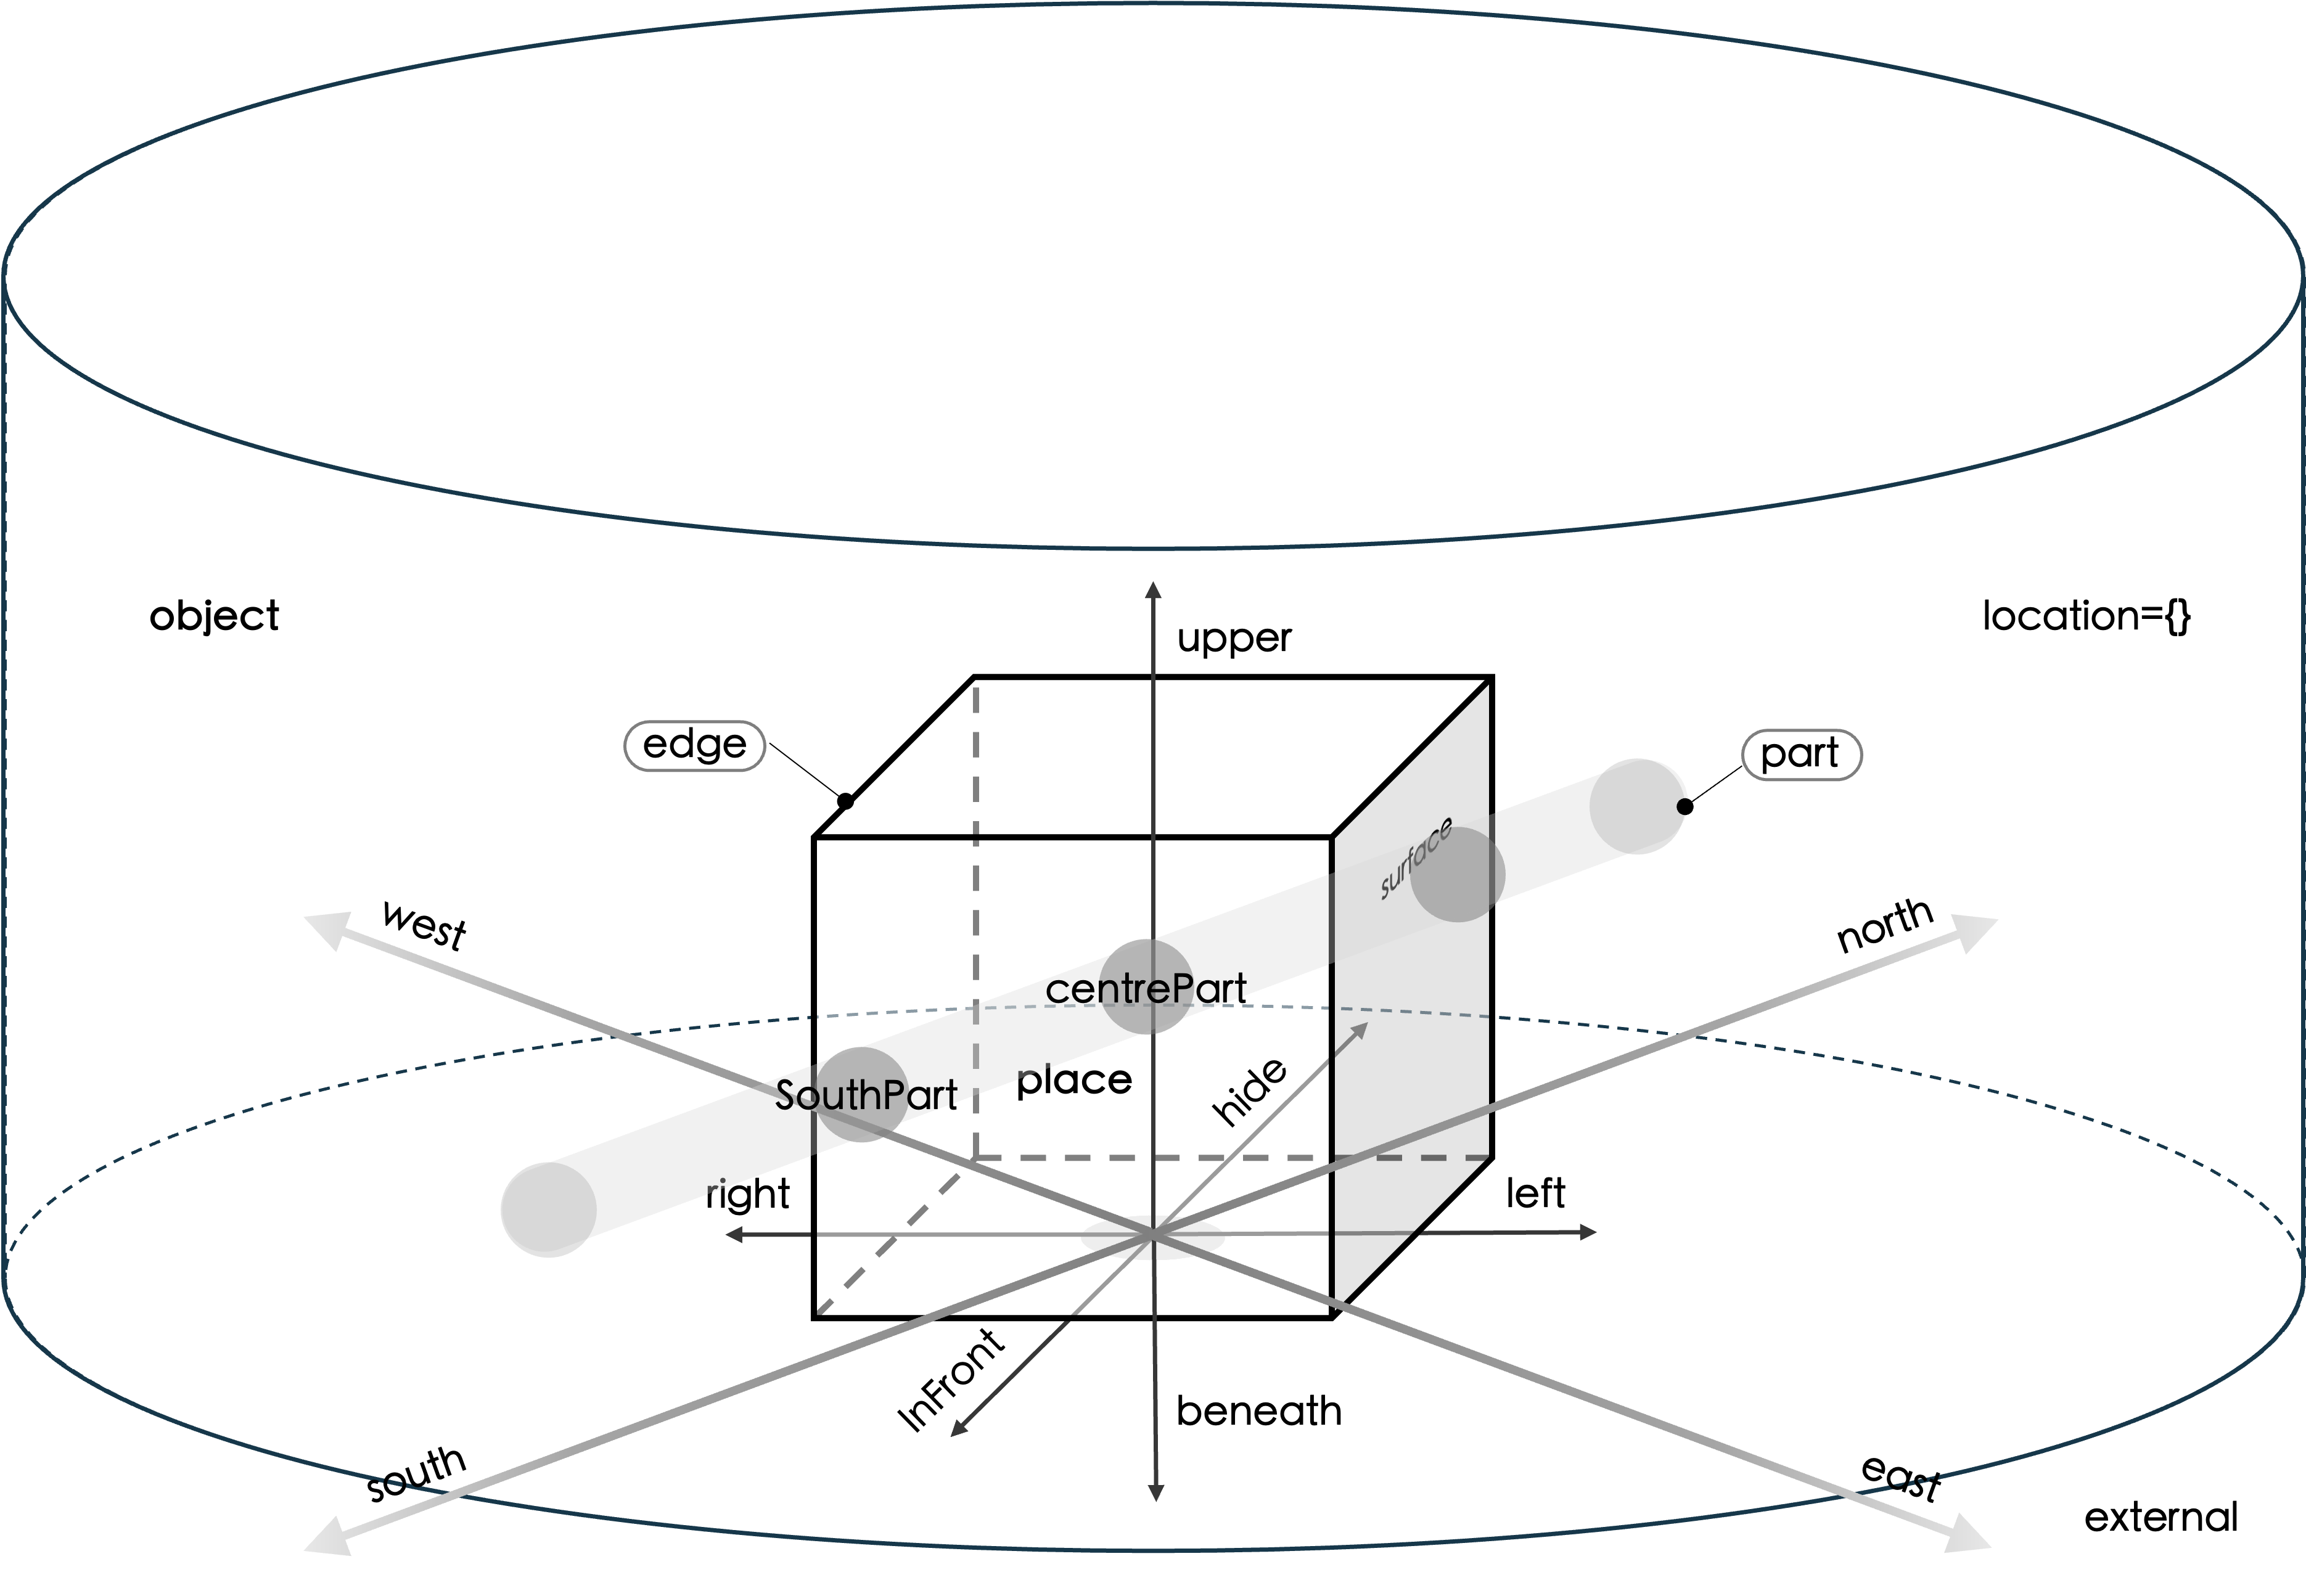
\includegraphics[width = \textwidth]{figures/spatialpreposition.png}
\caption{空間介詞與方位詞之語意圖(改自\citet{RN45})}
\label{fig:spatialpreposition}
\end{figure}


綜合上述討論,圖10顯示本研究發展之位置描述知識本體的空間介詞與方位詞及其概念串接至上層知識本體的結構。詳細來說,在\textit{locd:SpatialConcpet} (空間概念)下記錄\textit{locd:SpatialRelationship} (空間關係),依據E-HowNet之定義可再進一步細分為三個主要與位置表達相關的類別,分別為\textit{ehn:LocationFunction} (位置函數)、\textit{ehn:DistanceValue}和\textit{ehn:AlterLocation} (變空間位置)。

與空間概念關係相對的,在\textit{locd:LocationDescription}相關的兩個類別\textit{locd:SpatialPreposition}和\textit{locd:Localizer}會記錄E-HowNet的詞彙資訊,又以E-HowNet中對於詞意作為細分,對應著\textit{locd: SpatialRelationship}的各個類別組成,例如:\textit{ehn:NortheastPartLocaliser} (東北部)對應著\textit{ehn:NorthPart}和\textit{ehn:EastPart},又\textit{ehn:東北部}會作為\textit{ehn: NortheastPartLocaliser}當中的一個實例。如此一來,表 7之清單會以知識本體形式記錄下,以供後續語意查詢與語意規則推論機制。

\section{空間認知三階段規則}

為了實現位置描述的自動化從空間資料中產生,本研究建構明確且可執行的空間認知三階段規則。這些規則能夠係透過位置描述知識本體橋接O-SLD三層式框架,進而支持情境感知的語意推論與產生語意式的位置描述。在本研究的建構之規則知識,以語意網規則語言(semantic web rule language, SWRL)的方式紀錄,並分為三個階段:情境影響參考物、資料層到語意層和語意層到自然語言層(參見表 8),這三個階段共同構成一套可擴充且具備語意解釋能力的推論框架,為後續位置詞彙的生成提供知識基礎。

\subsection{情境影響參考物選擇}

第一階段聚焦於情境如何影響參考物的選擇,在空間資料中,參考物類別繁多,然而在特定情境下,並非所有參考物皆具備語意位置描述的價值。因此,本階段的目的為根據情境,自動篩選出在該情境下具參考價值的空間物件類別,並賦予其語意角色,以利後續的語言生成與推理。舉例而言,在交通情境中,偏好識別道路及道路相關的空間物件,而忽略如海域、山脈或水體等地物。

本研究在位置描述知識本體中定義了情境(如交通和災防告警)與Feature類型(如建物和山脈等)都被記錄並形式化於知識本體中,在此階段的推論中,將透過SWRL規則對不同物件給定「參考物(\textit{locd:GroundFeature})」角色,以支持後續的推論中連結到參考物及其性質。例如:

\begin{lstlisting}[language=Prolog, basicstyle=\ttfamily, xleftmargin=2em]
Traffic(?ctx)^Road(?ref)^SpatialOperation(?rel) 
->GroundFeature(?ref)^hasGroundFeature(?rel, ?ref)
\end{lstlisting}

此規則表示,在Traffic (交通情境)下,Road (道路)視為GroundFeature (參考物件)這個角色。
除情境規則外,亦可擴充不依賴特定情境或物件之通用規則,例如:

\begin{lstlisting}[language=Prolog, basicstyle=\ttfamily, xleftmargin=2em]
GeneralContext(?ctx)^Feature(?ref)^SpatialOpeartion(?rel)
->GroundFeature(?ref)^hasGroundFeature(?rel, ?ref)
\end{lstlisting}

此規則表示,只要是Feature (圖徵)即是GroundFeature (參考物件)這個角色。

\subsection{資料層到語意層}

第二階段聚焦於空間語意的推論,此階段的目的是將空間物件與各類空間操作合理轉化為語意上的空間關係,進而為後續產生位置描述提供基礎。舉例而言,對於語意上的空間關係「Upper」,若參考物為「建物」與「公園」,在人類解讀上可能會產生不同的語意。若參考物改為「建物」,「Upper」則可能指目標物在建物頂樓上方,且這樣的空間關係是具有普遍性,對於建物大多能達成。然而,若「公園」為參考物,日常鮮少會描述自己位於公園「上」,因此若無考量參考物之語意,可能會造成不合理的推論結果。

在此階段中,透過 SWRL 規則對不同類型的Feature及其語意進行推論,以確保語意層的合理性與準確性,本研究將設計一組關鍵空間操作通用規則集,包括「Intersects」和「Touches」等空間操作,例如:

\begin{lstlisting}[language=Prolog, basicstyle=\ttfamily, xleftmargin=2em]
Within(?rel)^FigureFeature(?tar)^hasFigureFeature(?rel, ?tar)
^GroundFeature(?ref)^hasGroundFeature(?rel, ?ref)
->OnSite(?rel)
\end{lstlisting}

此規則表示,在目標物與參考物存在GIS空間操作「Within」,則視為語意上的空間關係「OnSite」。
此外,根據特性考慮結合Feature性質(主要為幾何類型、類別和其他性質),以達成無法直接從空間操作中描述的語意空間關係,例如:

\begin{lstlisting}[language=Prolog, basicstyle=\ttfamily, xleftmargin=2em]
Within(?rel)^FigureFeature(?tar)^hasFigureFeature(?rel, ?tar)
^GroundFeature(?ref)^hasGroundFeature(?rel, ?ref)
^hasQuality(?ref, ?form)
^StyleandForm(?form)^qualityValue(?form, “elevated”)
->Upper(?rel)
\end{lstlisting}

此規則表示,在目標物與參考物存在GIS空間操作「Within」,且當參考物存在StyleandForm(型態)為「elevated(帶有高程)」時,則視為語意上的空間關係「Upper」,以此來建構具語意合理性的推論。

綜述而言,該階段透過知識本體與SWRL規則的結合,確保空間語意推論結果的合理性,既能反映Feature之間的真實關係,又能符合人類語意表達的邏輯與常識。

\subsection{語意層到自然語言層}

第三階段的重點是將語意層的推論結果轉化為自然語言描述,以實踐產生自然語言形式的位置描述。本階段的目標是產生能夠符合人類閱讀與解釋習慣的自然語言描述,同時保持語意的一致性與精確性。為提升自然語言生成的靈活性,本研究將採用基於模板(template-based)的生成方法,結合情境化規則進行描述細化。在語意轉化過程中,將結合 SWRL 推論結果與自然語言生成(natural language generation, NLG)技術,逐步將知識本體中的語意規則映射至語意結構,例如:

\begin{lstlisting}[language=Prolog, basicstyle=\ttfamily, xleftmargin=2em]
OnSite(?rel)^LocationDescription(?locad)
^symbolize(?rel, ?locad)^AtSpatialPreposition(?word)
->hasSpatialPreposition(?locad, ?word)
\end{lstlisting}

此規則表示,當存在空間關係為「OnSite」時,會推得出 AtSpatialPreposition (「在」的空間介詞),因此 LocationDescription (位置描述)可獲得空間介詞為「在」。

\section{情境分析}

在交通相關的情境中,知識本體需能表示的不僅是道路的類型,還包括道路段、交叉路口與附屬設施。為了回應真實世界情境與領域語意的需求,本研究個案擴充了LocD本體,納入更細緻的道路網系統分類,這在交通情境中扮演關鍵角色。

知識本體中空間要素的基本分類依據內政部發布的《地形圖資分類架構》。為了彌合通用分類與情境中領域專屬類型間的落差,本研究引入交通部發布之《交通網路基本資料標準(第一版)》,該標準定義了臺灣交通系統的結構。此分類已整合至LocD本體作為其子結構,如圖六所示。

這些交通情境與對應的參考物件也進一步連結至第 3.3 節所述的具情境感知之推論規則,使系統在語意推理過程中能動態決定符合情境的參考物件。基於警察廣播電台(PBS)提供的 2,000 筆即時交通通報資料,本研究應用實體命名辨識(NER)技術,將原始的非結構化資料轉換為結構化格式,並進行本體語意標註,藉此識別在交通語境中常被使用的參考物件類型。

\begin{lstlisting}[language=Prolog, basicstyle=\ttfamily, xleftmargin=2em]
SpatialOperation(?rel)^hasContext(?rel, ?ctx)^Traffic(?ctx)
^Feature(?f)^hasFeature(?rel, ?f)^hasQuality(?f, ?type)
^UndergroundUrbanRoad(?type)^FigureFeature(?ff) 
->hasFigureFeature(?rel, ?ff)
^GroundFeature(?f)^hasGroundFeature(?rel, ?f)
\end{lstlisting}


\section{評估方法}
本研究採用SPICE(Semantic Propositional Image Caption Evaluation)作為評估指標\citep{RN29},以衡量機制產生之候選描述與參考描述之間的語意對齊程度。相較於傳統以字串層級為主的評估指標(如BLEU和ROUGE),或近年來基於大型語言模型之語意層級評估指標(如BERTScore),SPICE 能更準確反映語句的語意結構及實體匹配,適合本研究所關注之語意式位置描述任務。

SPICE主要以F1 score作為核心指標,綜合考量語意單元的準確率(Precision)與召回率(Recall)。語意單元係指候選與參考描述文字透過語意場景圖(semantic scene graphs)分析後所產生的三元組(triple)集合,其形式為「(object)」、「(object, attribute)」、「(object, relation, object)」三者。其中,準確率表示機制產生的語意單元中,有多少與參考描述一致;召回率則反映參考描述中的語意單元,有多少被機制成功捕捉;F1 分數則為兩者的調和平均,用以綜合評估語意重合程度。其數學定義如下(式1-1至1-3),其中準確率為$P$、召回率為$R$,$c$為候選文字、$S$為參考文字、$T(G(c))$為候選三元組集合、$T(G(S))$為參考三元組集合,而$\otimes$意味集合匹配與否。

在本研究之任務中,語意單元統一定義為「(空間介詞, 地點名稱, 方位詞)」之三元組形式,例如:位置描述「在中山高速公路上」將被轉換為「(在, 中山高速公路, 上)」的三元組。為確保評估準確性與參考資料的一致性,本研究之參考描述之真值(ground truth)經由個案分析後人工標記產生,經人工語意理解後轉換為三元組形式。

此外,為處理同地異名和同義詞情況,本研究建立了地理實體對應辭典,以統一地點名稱的語意指涉,例如:「中山高速公路」、「國道一號」或「國1」等應視為指涉相同地理實體。同時,針對空間介詞及方位詞的匹配操作,本研究採用E-HowNet中文詞庫作為語意相似度的判斷依據,例如:「位於」和「在」在E-HowNet上會視為是同義詞。基於SPICE指標結合地理辭典與中文詞庫,本研究提升了三元組匹配的語意靈敏度與評估準確性。


